\documentclass{article}
\usepackage[utf8]{inputenc}
\usepackage{geometry}
\usepackage{graphicx}
\usepackage{hyperref}

\geometry{
left=25mm,
right=25mm,
top=20mm,
bottom=25mm
}

\title{\textbf{Report N°5 MSc Thesis: Active Constraints}\newline \large{\textit{Recap of Phase 1}}}
\author{\textbf{Alberto Rota} - \textit{Supervisor: Prof. Elena De Momi}}
\date{}

\begin{document}
\maketitle
\paragraph{Title:} \textit{To Be Defined}
\section*{General guidelines}
    Development of surgical training tasks implementing Active Constraints of
    different nature and with different levels of intervention, in order to
    evaluate their efficacy and role in Robot-Assisted Minimally Invasive Sugery.
    \begin{itemize}
        \item \textit{Phase 1: }Software Development in a virtual environment (Unity)
        \item \textit{Phase 2: }Implementing on the dVRK, followed by
        experimental tests with data gathering, analysis and validation
    \end{itemize}

\noindent With this report I'll summarize all the work that went into Phase 1 of the project. I'm considering this phase as concluded as a number of task implementing virtual fixtures have been constructed and (beside only indirectly) tested. Next would be the deployment of such tasks to the dVRK in the LAB, followed by the esperimental evaluation of their practical effectiveness.

\section*{The tasks}
\begin{figure}[h!]
    \centering
    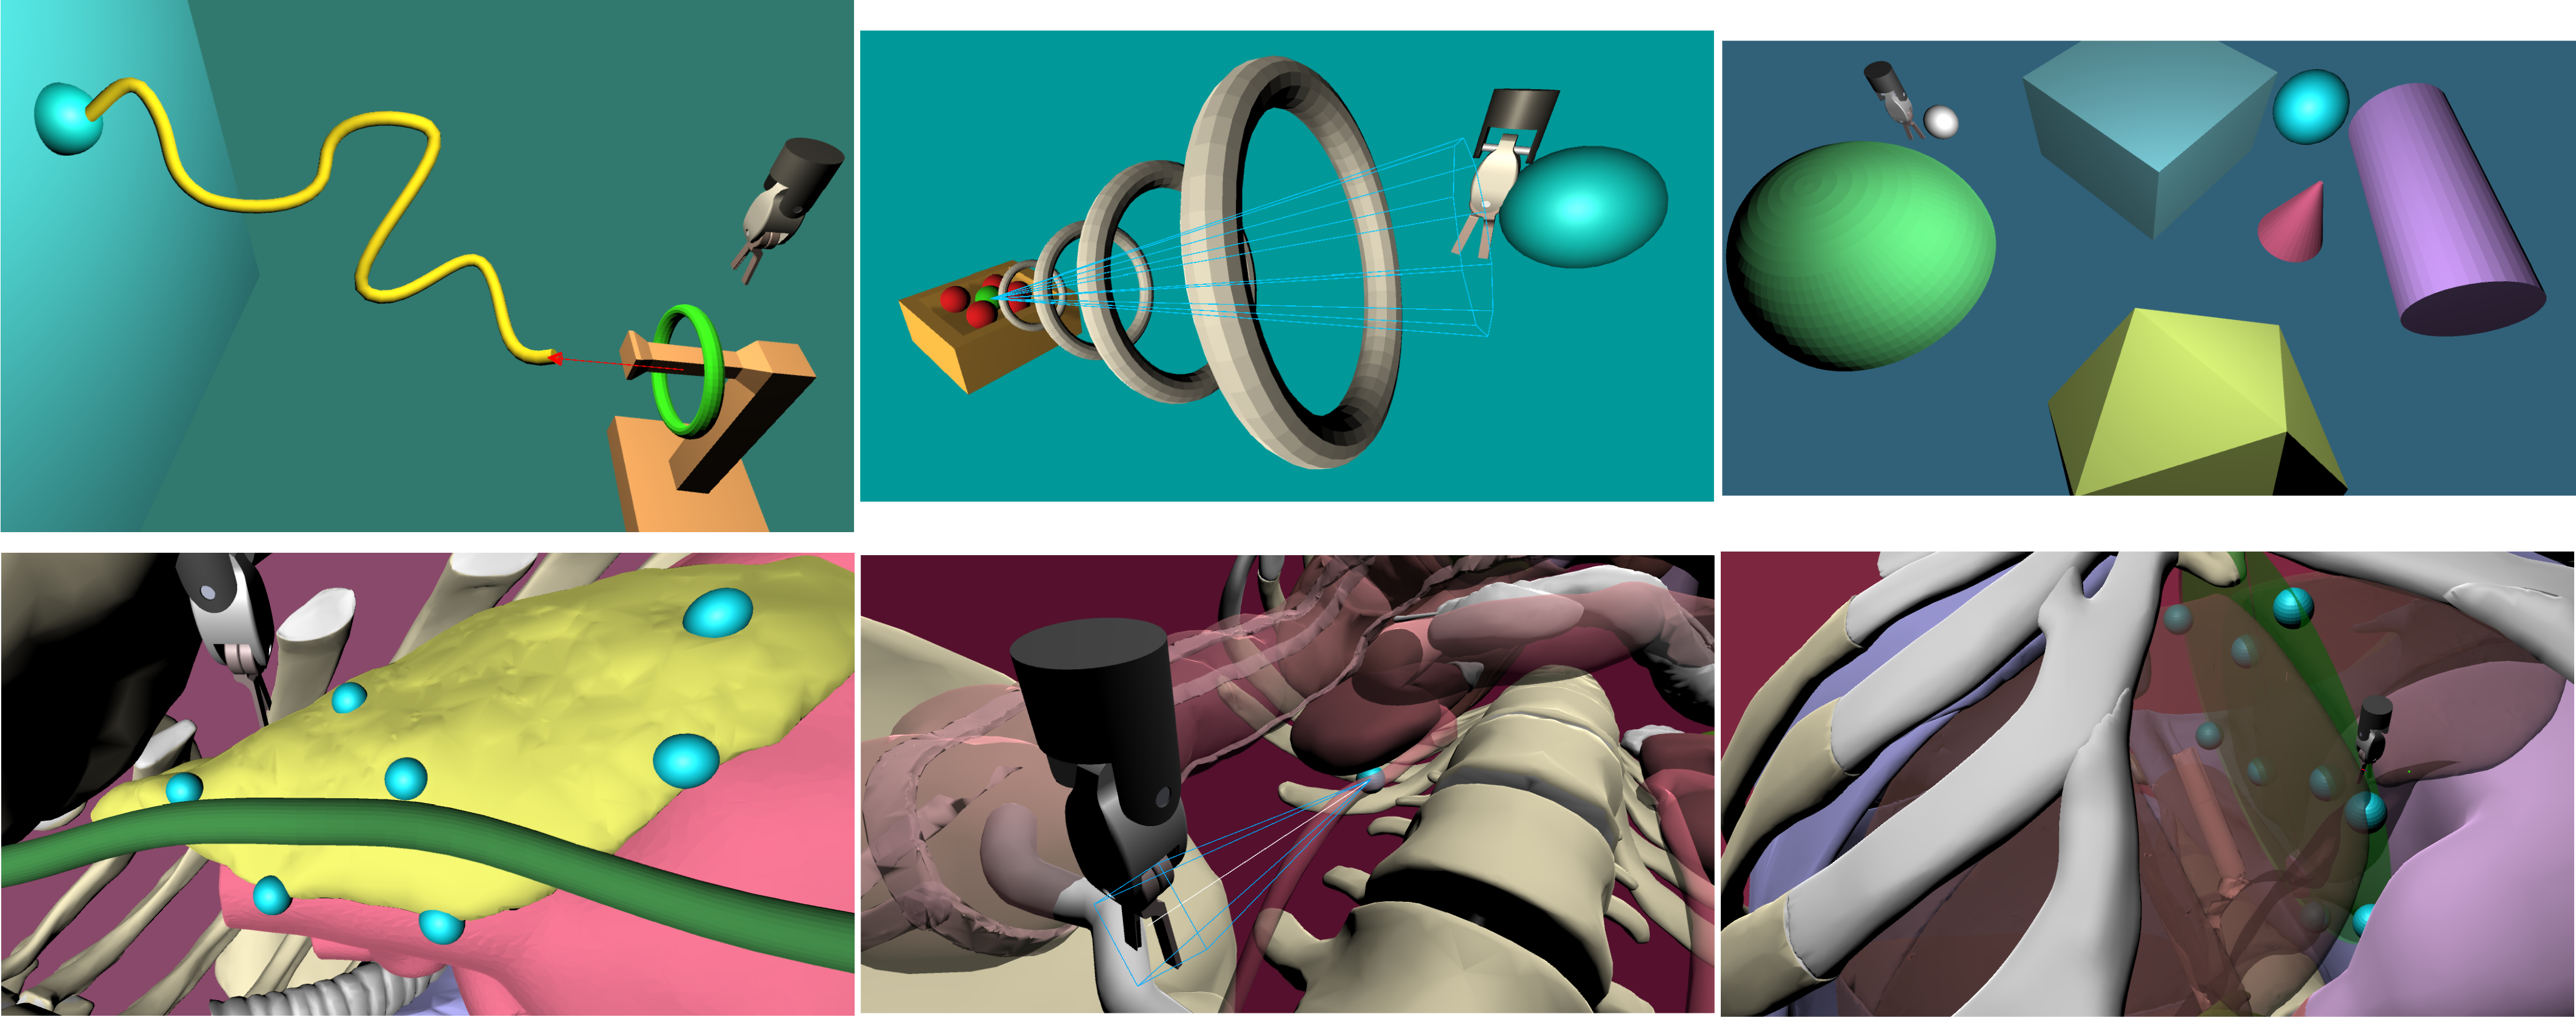
\includegraphics[width=\textwidth]{tasks.png}
\end{figure}

\noindent \textbf{Watch the video if you don't want to read a more verbose explaination later: }\newline At the link \href{https://we.tl/t-xs9iOlAxx0}{https://we.tl/t-xs9iOlAxx0} there is a 1.5 minutes video with brief snapshots of each task in progress. For testing purposes, I've been driving the movement of the PSM with my keyboard (W key = forward, S key = backwards, \textit{etc.}) and the force is applied directly to the PSM. In the experimental case this will not be the case, as the force will be experienced as anhaptic feedback on the MTM.

\newpage
\noindent 6 total tasks have been build, 3 regarding surgical training (top row of the figure) and 3 regarding surgical operations in real scenarios when Robot-Assisted Minimally Invasive surgery is employed(a Thymectomy, a Nephrectomy and a Liver Resection, bottom row of the figure).
\begin{itemize}
    \item \textbf{Training 1: Ring through a curve:} The subject pinches the ring with the PSM and must carry it to the target (blue sphere) following the curved path.\newline
    \phantom{.....}\textit{Employs a Trajectory Guidance Virtual Fixture}

    \item \textbf{Training 2: Extraction of a target:} The subject must approach the target (green sphere) without making contact with the 4 rings, then he must grab it and bring it back to the starting position. \newline
    \phantom{.....}\textit{Employs a Conical Containement Virtual Fixture}

    \item \textbf{Training 3: Obstacle Avoidance:} The subject pinches the white sphere and brings it to the target blue sphere without touching the obstacles. \newline
    \phantom{.....}\textit{Employs an Obstacle Avoidance Virtual Fixture}

    \item \textbf{Thymectomy:} The subject must pinch several points around the thymus gland (yellow) without making contact with the phrenic nerve (green)\newline
    \phantom{.....}\textit{Employs a Obstacle Avoidance Virtual Fixture}

    \item \textbf{Nephrectomy:} The subject must approach the renal pelvis without making contact with the other organs.\newline
    \phantom{.....}\textit{Employs a Conical Containement Virtual Fixture}

    \item \textbf{Liver resection:} The subject must pinch a number of targets positioned along the demarcation plane of two liver lobes\newline
    \phantom{.....}\textit{Employs a Surface Guidance Virtual Fixture}
\end{itemize}
    
\section*{Evaluation protocol}
The evaluation phase should aim at evaluating if such virtual fixtures provide effective aid when performing the tasks, therefore I would conduct the evaluation as follows (for each task):
\begin{enumerate}
    \item The subject performs the task unassisted, "switching off" the virtual fixture.
    \item The subject performs the task assisted by the virtual fixture haptic feedback force
    \item The subject performs the task unassisted once more
\end{enumerate}
We should see an improvement in the task performance quality from 1 to 2, but also from 1 to 3. To assess the task performance quality, a few evaluation parameters are extracted when the subject has completed the task, in particular:
\begin{itemize} 
    \item \textbf{Task duration:} The time it took the subject to complete the task.
    \item \textbf{Average distance:} The average distance between the subject and the reference trajectory/surface or from the obstacles.
    \item \textbf{Average force:} The average force feedback applied to the subject.
    \item Other parameters can be added later.
\end{itemize}
These parameters are computed automatically. The task data is logged and "recorded" automatically from Unity in .csv files: everything is logged (position and velocity of the PSM over time, haptic feedback force over time, reference trajectories, position and extents of obstacles, \textit{etc.}). 
\newline

\noindent A number of volunteer subjects will be recruited to perform the tasks: a statistical significance test will be performed to finally assess the effectiveness of virtual fixtures is robotic surgery.
\newline

\noindent \textbf{My repository on GitHub: }\href{https://github.com/alberto-rota/MSc-Thesis-Active-Constraints-in-RAMIS}{https://github.com/alberto-rota/MSc-Thesis-Active-Constraints-in-RAMIS}
\end{document}